\documentclass[12pt]{spieman}  % 12pt font required by SPIE
\usepackage{amsmath,amsfonts,amssymb}
\usepackage{graphicx}
\usepackage{setspace}
\usepackage{tocloft}
\usepackage{lineno}
\usepackage{booktabs}
\usepackage{xcolor}
\linenumbers
\DeclareMathOperator*{\argmin}{arg\,min}

% ---------------------------------------------------------------
% Drafting helpers -- REMOVE BEFORE SUBMISSION
% ---------------------------------------------------------------
\newcommand{\todo}[1]{\textcolor{red}{[TODO: #1]}}

\title{Preserving lesion quantification in longitudinal whole-body PSMA PET/CT registration}

\author[a,b,c,*]{Fryderyk K{\"o}gl}
\author[a,b,c]{Anna Reithmeir}
\author[a]{Daniel M. Lang}
\author[a,b]{Emily Chan}
\author[d]{Lukas F{\"o}rner}
\author[e]{Rickmer Braren}
\author[a,b,c,f]{Julia A. Schnabel}
\affil[a]{Helmholtz Munich, Neuherberg, Germany}
\affil[b]{Technical University of Munich, Munich, Germany}
\affil[c]{Munich Center for Machine Learning, Munich, Germany}
\affil[d]{University Hospital Augsburg, Department of Diagnostic and Interventional Radiology and Neuroradiology, Augsburg, Germany}
\affil[e]{University Medical Center Hamburg-Eppendorf, Hamburg, Germany}
\affil[f]{King's College London, London, United Kingdom}

\renewcommand{\cftdotsep}{\cftnodots}
\cftpagenumbersoff{figure}
\cftpagenumbersoff{table}
\begin{document}
\maketitle

\begin{abstract}
\textbf{Purpose:} \todo{One or two sentences: longitudinal PSMA PET/CT registration should align anatomy without altering lesion volume and uptake.}

\textbf{Approach:} \todo{LapIRN + instance optimisation with PET-preservation and bone-rigidity losses; patient-level split; comparison with NiftyReg and ConvexAdam; ablations of where the losses act.}

\textbf{Results:} \todo{Main numbers after all experiments are in: accuracy vs.\ baselines, MTV/TLG change with and without the losses, IO-only placement, per-lesion effect for small bone lesions.}

\textbf{Conclusions:} \todo{One or two sentences.}
\end{abstract}

\keywords{deformable image registration, PSMA PET/CT, longitudinal imaging, biomarker preservation, instance optimization}

{\noindent \footnotesize\textbf{*}Fryderyk K{\"o}gl, \linkable{fryderyk.koegl@tum.de}}

\begin{spacing}{2}

\section{Introduction}
\label{sect:intro}

Prostate-specific membrane antigen (PSMA) PET/CT is now routinely used for staging prostate cancer, for planning and following radioligand therapy, and for assessing treatment response~\cite{ref_psma_clinical}.
In such longitudinal imaging, patients are scanned before therapy (baseline) and again at one or more follow-up time points.
Registering each follow-up image to the baseline image makes it possible to compare tumor burden voxel by voxel or track individual lesions over time~\cite{ref_psmareg_challenge}.
For these uses, a registration has to align the anatomy while preserving the PET-derived quantities of the warped image.
Two such quantities, under the names used by the Learn2Reg 2026 PSMAReg challenge~\cite{ref_psmareg_challenge}, are the metabolic tumor volume (MTV) and the total lesion glycolysis (TLG); for PSMA PET, they measure the PSMA-positive tumor volume and the total lesion PSMA uptake.
A deformation that compresses or stretches a lesion would change both these quantities and thereby introduce a registration-induced bias into the measured longitudinal change.
When the registered follow-up is used to match lesions or compare them with baseline, such processing-induced changes could be mistaken for part of the longitudinal change and could therefore affect lesion tracking or response assessment.
The challenge, part of the Learn2Reg series~\cite{ref_learn2reg_hansen,ref_learn2reg_alessa} and based on the PSMA-PET-CT-Lesions dataset~\cite{ref_psmaregdata}, formalizes this setting by registering each follow-up image to its baseline image with a dense deformation field.
It scores organ overlap, boundary distance, folding of the deformation field, and the change of MTV and TLG caused by the deformations.
Anatomical alignment and the preservation of these quantities can compete: limiting deformation may protect lesion measurements while leaving the anatomy misaligned, whereas improving alignment may distort the lesions being measured.

Classical registration solves an optimization problem per image pair~\cite{ref_demons,ref_syn,bspline}; this can be accurate~\cite{ref_learn2reg_alessa,ref_learn2reg_hansen}, but it is often computationally expensive, in particular for large three-dimensional whole-body images~\cite{ref_voxelmorph_cvpr}.
Learning-based registration amortizes this optimization: a network is trained once on many image pairs and then registers a new pair in a single forward pass~\cite{ref_voxelmorph_tmi,ref_svf_voxelmorph,ref_transmorph}.
Instance optimization (IO) refines the network's deformation field for each image pair by classical iterative optimization at test time.
Whole-body images of the same patient can differ by large deformations, for example through different positioning of the arms, spine, and bowel.
We therefore build on LapIRN~\cite{ref_lapirn}, a learning-based method that estimates the deformation coarse to fine on a Laplacian image pyramid.
Its coarse levels recover large deformations and its finer levels add smaller ones, while the transformation remains smooth and invertible.
With a network and optional IO, preservation constraints can act during training, during per-pair refinement, or at both stages; the choice affects both registration quality and runtime.
The label-guided IO studied here uses predicted organ and lesion masks for each pair; we evaluate its output against the provided labels.
Its PET-preservation losses act on the predicted lesion mask, so a lesion absent from that mask receives no direct preservation constraint.

Our earlier Learn2Reg submission introduced the affine--LapIRN--IO pipeline with PET-preservation and per-bone rigidity losses~\cite{ref_koegl_arxiv}.
It evaluated selected configurations on challenge validation cases using surrogate labels.
In this extension, we retrain on a new patient-level split of the released labeled cohort and reserve 28 patients for final evaluation.
We add controlled loss-placement comparisons, tuned baselines, patient-level statistics, and per-lesion analyses.
These 28 patients were among the challenge data available during development of the earlier method, so the split provides a holdout for the present analyses rather than an independent external cohort.

First, we ask whether the PET-preservation and bone-rigidity losses reduce registration-induced change and what alignment accuracy they cost, both with and without IO.
We then ask whether applying the losses only during IO can recover the preservation obtained by also using them in training, and compare that choice with the faster network-only setting.
Finally, we analyze changes to individual lesions and the coverage of the predicted lesion masks used by IO to understand what limits preservation.
Because many PSMA lesions lie in bone, we also compare rigidity penalties for low-resolution whole-body CT, where thin skeletal structures make local constraints difficult to apply.
Our contributions are:
\begin{itemize}
  \item We compare PET-preservation and rigidity losses during network training, IO, or both.
  Loss-guided IO improves alignment without a detected increase in image-level MTV or TLG change relative to network output, and applying the losses only in IO gives higher alignment accuracy than using them at both stages.
  \item We analyze the remaining change.
  Missed lesions account for most of the residual image-level PET change in the mask-coverage analysis, while image-level MTV and TLG hide substantial changes to individual lesions even when provided masks are used.
  \item We compare rigidity penalties for whole-body CT.
  A per-bone rigid fit avoids the boundary leakage of finite-difference penalties and the loss of skeleton under erosion, and yields the lowest within-bone distance distortion among the tested penalties.
  \item We provide a patient-level evaluation with the official challenge scorer, a selection rule that weighs preservation against a fixed Dice tolerance, and tuned NiftyReg and ConvexAdam baselines.
\end{itemize}

\begin{figure}
\begin{center}
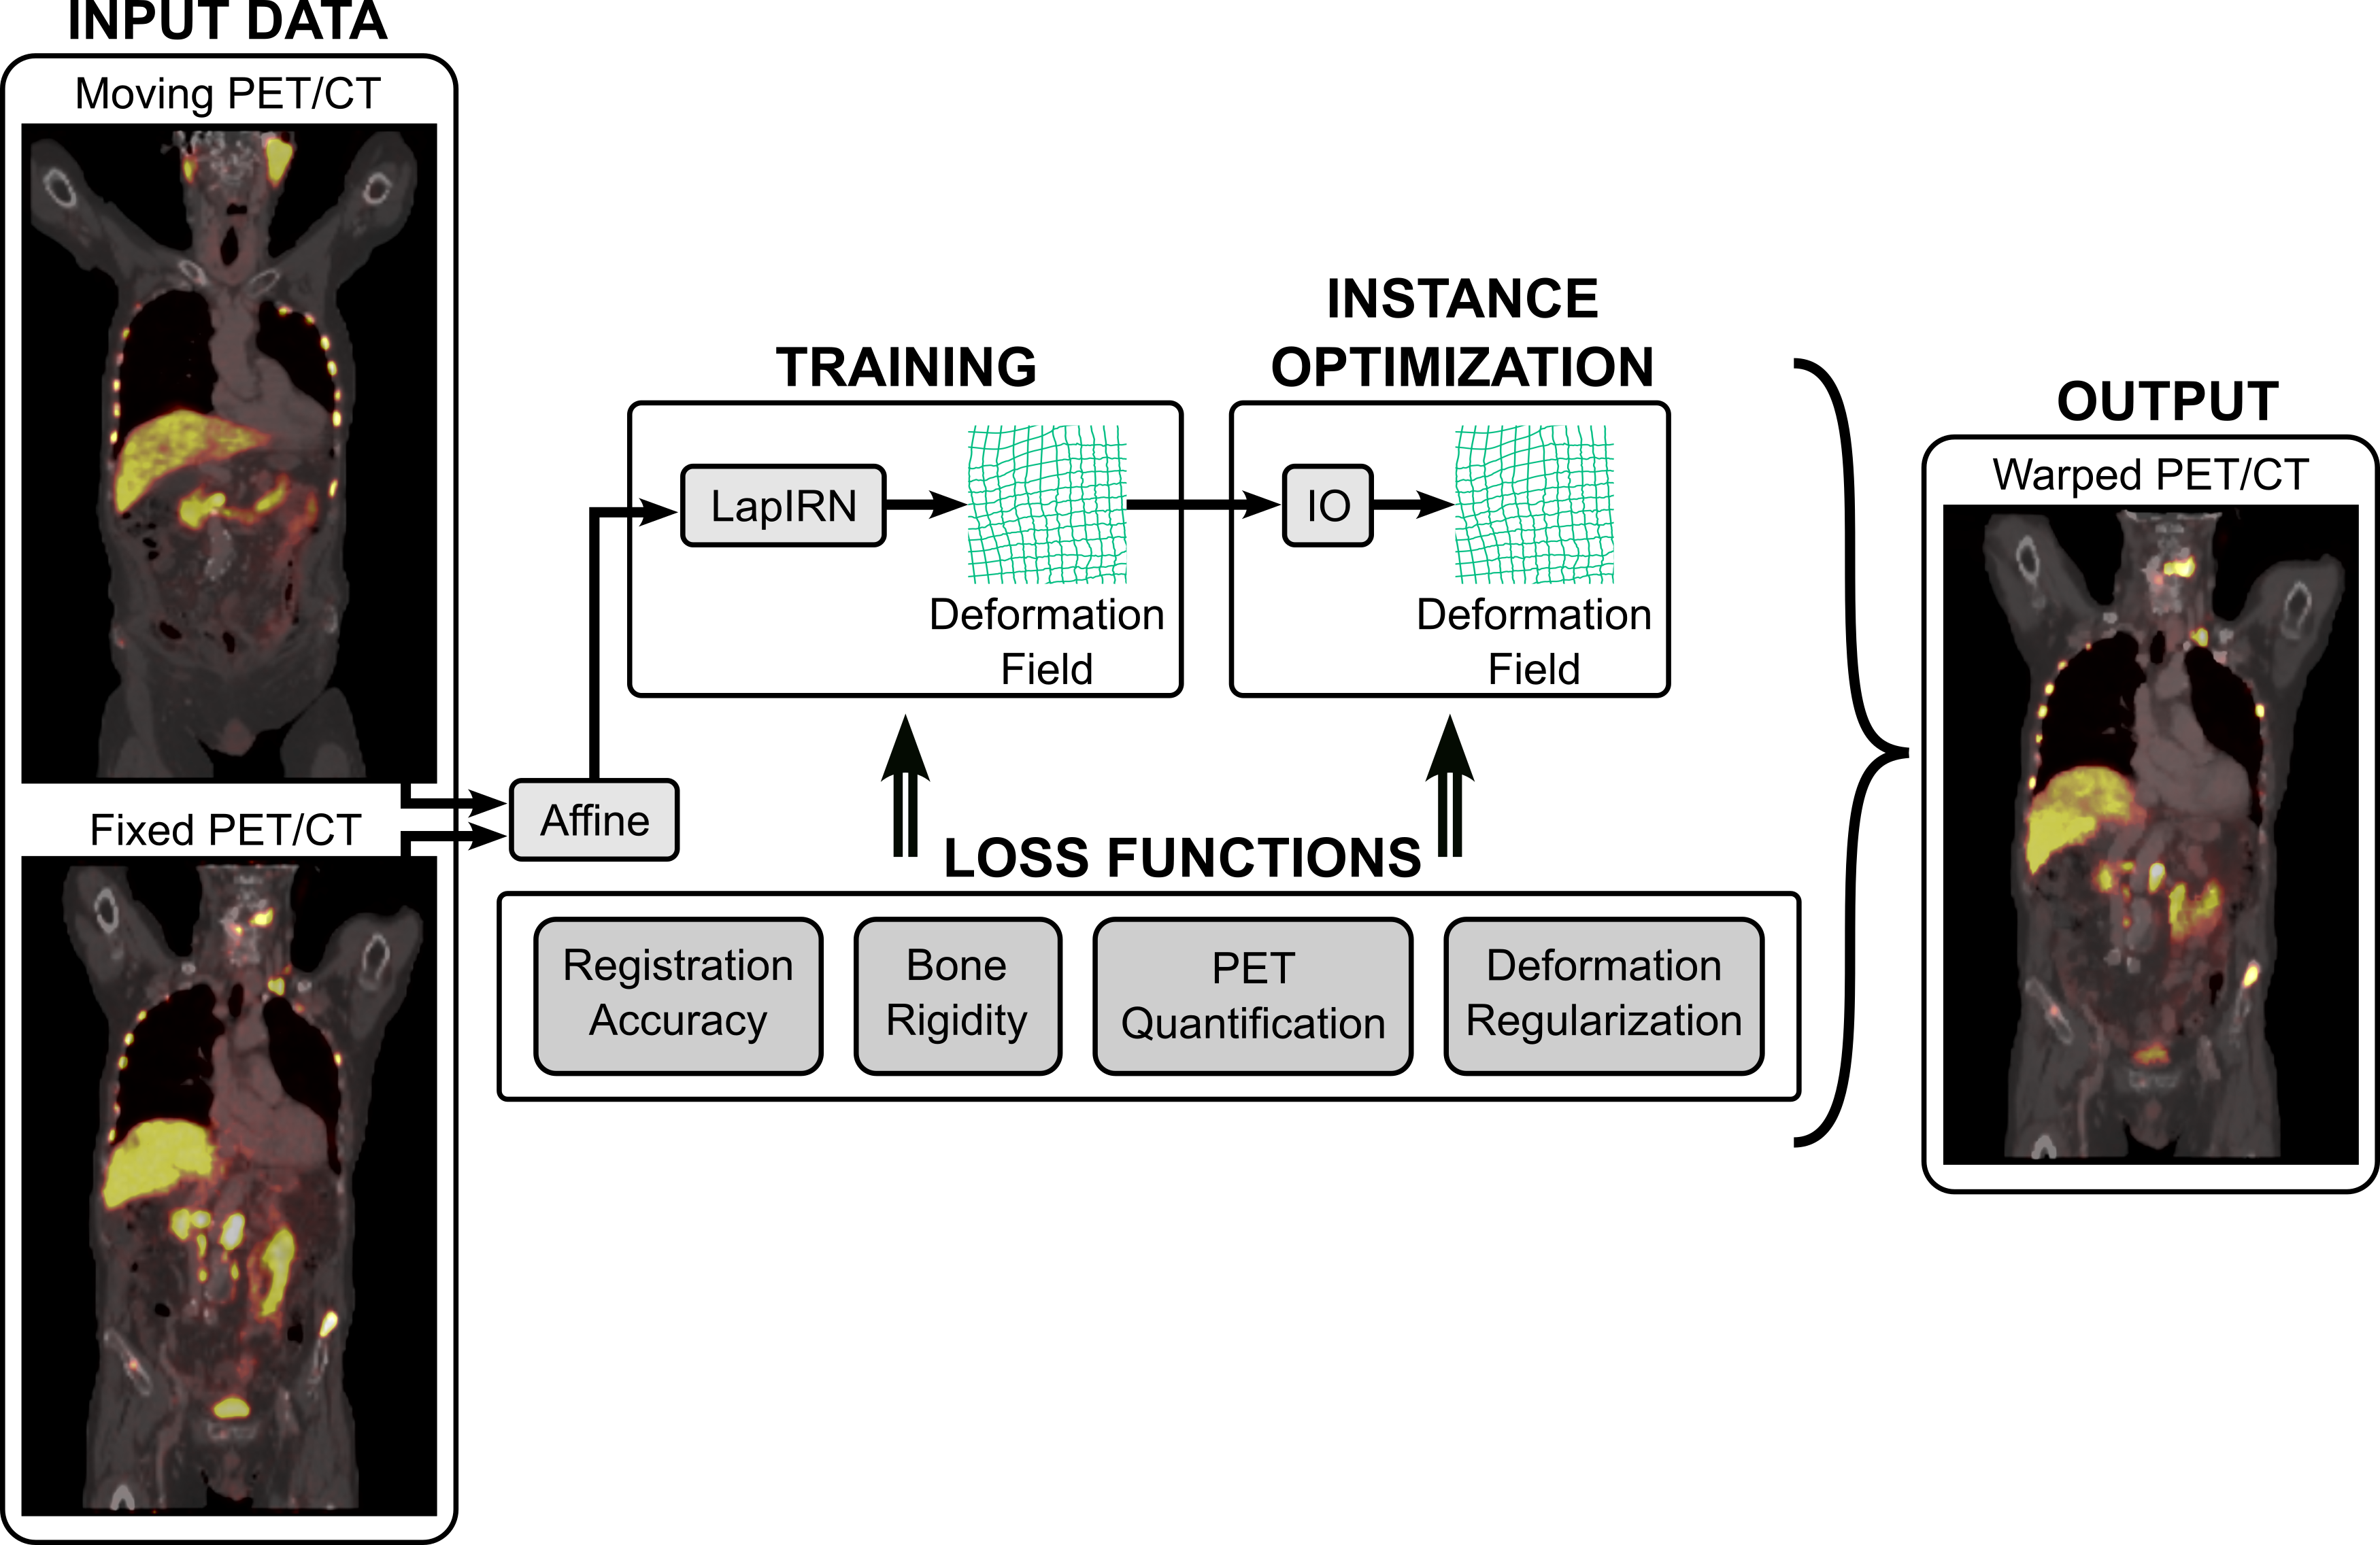
\includegraphics[width=\linewidth]{figures/overview.png}
\end{center}
\caption{\label{fig:pipeline}
Registration pipeline.
The follow-up (moving) and baseline (fixed) PET/CT images are aligned by an affine pre-registration, then by the LapIRN network, which predicts a dense deformation.
Instance optimization (IO) refines this deformation per pair before the moving image is resampled into the fixed frame.
Network training and IO use the same groups of loss terms: registration accuracy, bone rigidity, PET quantification, and deformation regularization (Sec.~\ref{sect:objective}).
The bone-rigidity and PET-quantification terms can be used in training, in IO, or in both; our method uses them only in IO.}
\end{figure}

\section{Methods}
\label{sect:methods}

\subsection{Data and Split}
\label{sect:data}

We used the training set of the PSMAReg challenge~\cite{ref_psmareg_challenge,ref_psmaregdata}, a longitudinal whole-body PSMA PET/CT cohort.
Each scan consists of a CT and a PET image (in SUV), resampled to $2.7344\times2.7344\times3.27$~mm and cropped to $192\times192\times288$ voxels.
For every scan, the challenge provides 117 CT organ labels (the TotalSegmentator~\cite{ref_totalsegmentator} classes) and a PSMA lesion mask.
Following the challenge, a follow-up scan is always the moving image and the corresponding baseline scan the fixed image.

We split the 146 labelled patients with at least two scans at the patient level into training, validation, and test sets, aiming at 70/15/15\,\% of the registration pairs and balancing the sets for tumour burden and for bone- versus soft-tissue lesion location.
Training uses all pairs of later onto earlier examinations of a patient; validation and testing use only follow-up-to-baseline pairs, as in the challenge.
This gave 92/26/28 patients and 178/38/38 pairs.
The split was built once with a fixed seed and frozen before any experiment of this study; all choices of settings, checkpoints, and methods were made on the validation set, and the test set was used only for the final evaluation.
All patients were part of the challenge training data used to develop the earlier version of the method~\cite{ref_koegl_arxiv}; the test patients were not used for any decision in the present study.

\paragraph{Labels used by the method and for evaluation.}
Instance optimisation (Sec.~\ref{sect:io}) needs organ and lesion labels of the test scans.
To keep evaluation independent of the inputs, IO uses only predicted labels: organ labels predicted by TotalSegmentator~\cite{ref_totalsegmentator} on the CT, and lesion masks predicted by an nnU-Net~\cite{nnunet} trained on the training patients only.
\todo{nnU-Net details: input channels, configuration, folds; lesion Dice on the validation set (about 0.55).}
The provided labels are used only for evaluation (Sec.~\ref{sect:metrics}).

\paragraph{Preprocessing.}
For the network and IO, CT was clipped to $[-1000,1500]$~HU and PET to $[0,20]$~SUV, and both were rescaled to $[0,1]$.
As in the ConvexAdam baseline of the challenge~\cite{ref_convexadam}, the patient bed was removed from the CT.
All PET quantities in the evaluation are computed on the original SUV images.

\subsection{Registration Pipeline}
\label{sect:pipeline}

The pipeline (Fig.~\ref{fig:pipeline}) has three stages, all estimated from the moving scan $(C_m, P_m)$ and the fixed scan $(C_f, P_f)$, where $C$ denotes CT and $P$ PET.
We denote the affine transform by $\varphi_{\mathrm{aff}}$, the network deformation by $\varphi_\theta$, and their composition, which maps the original moving scan to the fixed scan, by $\varphi$.

\paragraph{Affine pre-registration.}
ANTs~\cite{ants} estimates an affine transform from the two CTs, using body masks, a $[-1000,1000]$~HU window, half-resolution images, and Mattes mutual information.
It is converted to a dense displacement field.

\paragraph{Deformable network.}
We use LapIRN~\cite{ref_lapirn} with three pyramid levels at quarter, half, and full resolution.
Each level predicts a stationary velocity field that is added to the upsampled velocity of the coarser level and integrated by scaling and squaring~\cite{ref_arsigny} into $\varphi_\theta$.
Each level receives four channels: the fixed CT and PET and the affinely aligned moving CT and PET.
The levels are trained one after the other; a finer level is initialised from the coarser one, which is first kept frozen and then trained jointly.
\todo{Architecture: number of residual blocks and expansion of the final runs; confirm start channels.}

\paragraph{Instance optimisation.}
\label{sect:io}
At test time, the deformation of each pair is refined by optimising a residual stationary velocity field, initialised at zero and integrated by scaling and squaring (seven steps), on top of the total transformation $\varphi$.
The residual is optimised at full resolution with Adam~\cite{ref_adam} (learning rate $0.0125$, 40 iterations).
The objective is the same as in training (Sec.~\ref{sect:objective}), with the predicted labels in place of ground-truth labels.
Of the 40 iterates, we return the one with the lowest objective, in which the interpolated (soft) MTV and TLG terms are replaced by their nearest-neighbour (hard) values, i.e.\ by how the evaluation counts them; this selection uses only predicted labels.

\subsection{Registration Objective}
\label{sect:objective}

Network training and IO minimise a weighted sum of three groups of terms:
\begin{equation}
  \begin{aligned}
  \mathcal{L} = {} &
  \underbrace{\lambda_{\mathrm{NCC}}\mathcal{L}_{\mathrm{NCC}} + \lambda_{\mathrm{DSC}}\mathcal{L}_{\mathrm{DSC}}}_{\text{alignment}}
  + \underbrace{\lambda_{\mathrm{MTV}}\mathcal{L}_{\mathrm{MTV}} + \lambda_{\overline{J}}\mathcal{L}_{\overline{J}} + \lambda_{J}\mathcal{L}_{J} + \lambda_{\mathrm{TLG}}\mathcal{L}_{\mathrm{TLG}}}_{\text{PET preservation}} \\
  & + \underbrace{\lambda_{\mathrm{rig}}\mathcal{L}_{\mathrm{rig}} + \lambda_{\mathrm{smooth}}\mathcal{L}_{\mathrm{smooth}} + \lambda_{\mathrm{NDV}}\mathcal{L}_{\mathrm{NDV}}}_{\text{regularisation}} .
  \end{aligned}
  \label{eq:objective}
\end{equation}
All terms are evaluated on the total transformation $\varphi$.
The PET-preservation terms and the rigidity term are the subject of this study; they can be switched on in network training, in IO, or in both (Sec.~\ref{sect:experiments}).
The two coarse network levels never use them, because lesions and thin bones span only a few voxels at these resolutions.

\paragraph{Alignment.}
$\mathcal{L}_{\mathrm{NCC}}$ is the negative local normalised cross-correlation of the CTs, summed over one to three scales depending on the pyramid level.
PET is not used for similarity, because uptake changes between examinations with disease and therapy and a PET similarity would reward matching these changes.
$\mathcal{L}_{\mathrm{DSC}}$ is a soft Dice loss on the CT organ labels.

\paragraph{PET preservation.}
Let $M$ be the lesion mask of the moving scan and $\widetilde M$, $\widetilde P$ the linearly warped mask and PET.
Nearest-neighbour warping, as used in the evaluation, is piecewise constant in the displacement and gives no useful gradient; linear warping gives a soft lesion boundary instead.
The volume and uptake terms penalise the relative change caused by warping,
\begin{equation}
  \mathcal{L}_{\mathrm{MTV}} = \left(\frac{\left|\sum_x \widetilde M(x) - \sum_x M(x)\right|}{\sum_x M(x) + \epsilon}\right)^{2},
  \qquad
  \mathcal{L}_{\mathrm{TLG}} = \frac{\left|\sum_x \widetilde P(x)\widetilde M(x) - \sum_x P_m(x) M(x)\right|}{\sum_x P_m(x) M(x) + \epsilon},
  \label{eq:mtv_tlg}
\end{equation}
with $\epsilon=10^{-5}$.
Two further terms act on the Jacobian determinant $\det J_\varphi$ inside the warped lesion region $W$ in the fixed frame:
\begin{equation}
  \mathcal{L}_{\overline{J}} = \left(\frac{1}{|W|}\sum_{x\in W}\det J_\varphi(x) - 1\right)^{2},
  \qquad
  \mathcal{L}_{J} = \frac{1}{|W|}\sum_{x\in W}\bigl(\det J_\varphi(x) - 1\bigr)^{2}.
  \label{eq:jac_terms}
\end{equation}
$\mathcal{L}_{\overline{J}}$ constrains the net volume change of all lesions, and $\mathcal{L}_{J}$ additionally prevents compression in one part of a lesion from being compensated by expansion in another.
\todo{Confirm: in training, $W$ is the linearly warped mask for $\mathcal{L}_{\overline{J}}$ and the nearest-neighbour warped mask for $\mathcal{L}_{J}$, as in IO.}

\paragraph{Bone rigidity.}
Many PSMA lesions lie in bone, which moves rigidly between examinations.
For each of the 61 skeletal labels of the fixed scan (in IO: the predicted labels), we fit a rigid transformation to the displacement of the structure in closed form~\cite{ref_kabsch,ref_umeyama} and penalise the mean squared residual of its voxels; $\mathcal{L}_{\mathrm{rig}}$ is the mean over structures with at least 50 voxels.
Each bone is fitted independently, so neighbouring bones may move relative to each other, and the term involves no finite differences, so it does not constrain the tissue around a bone.

\paragraph{Regularisation.}
$\mathcal{L}_{\mathrm{smooth}}$ is the mean squared spatial gradient of the displacement.
$\mathcal{L}_{\mathrm{NDV}}$ is a differentiable version of the challenge's non-diffeomorphic volume, which splits every voxel into tetrahedra and accumulates the negative part of their Jacobian determinants~\cite{Liu2024}.

\paragraph{Weights.}
\todo{Table of $\lambda$ for training (full-resolution level) and IO. Training: $\lambda_{\mathrm{NCC}}=5$, $\lambda_{\mathrm{DSC}}=3/4/5$ per level, $\lambda_{\mathrm{smooth}}=10$, $\lambda_{\mathrm{NDV}}=10^4$, $\lambda_{\mathrm{MTV}}=5$, $\lambda_{\overline{J}}=0.125$, $\lambda_{J}=1.25$, $\lambda_{\mathrm{TLG}}=1.25$, $\lambda_{\mathrm{rig}}$ = ? IO (tuned, Sec.~\ref{sect:tuning}): $\lambda_{\mathrm{NCC}}=5$, $\lambda_{\mathrm{DSC}}=5$, $\lambda_{\mathrm{NDV}}=10$, $\lambda_{\mathrm{smooth}}=0$, $\lambda_{\mathrm{MTV}}=4\cdot10^4$, $\lambda_{\overline{J}}=10^3$, $\lambda_{J}=4$, $\lambda_{\mathrm{TLG}}=16$, $\lambda_{\mathrm{rig}}=0.25$. Confirm all training values against the final runs.}

\subsection{Rigidity Penalties Compared}
\label{sect:rigidity_methods}

Besides the per-bone rigid fit, we evaluate the rigidity penalty of Staring et al.~\cite{ref_rigidity_3_staring}, which requires the Jacobian $J$ inside a bone to be a rotation: $\det J = 1$, $J^{\top}J = I$, and vanishing second derivatives of the deformation.
It is computed with finite differences, whose stencil reads the 6 face and 12 edge neighbours of a voxel.
At a bone boundary, part of the stencil lies outside the bone, so the penalty also acts on the surrounding soft tissue or on a neighbouring bone.
A common remedy is to erode the bone mask so that the stencil stays inside; we erode each bone by exactly this 18-neighbour footprint, which removes the leakage completely.
The three variants (Staring, Staring with erosion, per-bone rigid fit) are compared in IO (Sec.~\ref{sect:experiments}).

\subsection{Training}
\label{sect:training}

Each level was trained with Adam~\cite{ref_adam}, a batch size of one, a linear learning-rate warm-up over five epochs, and a cosine decay to 10\,\% of the initial rate.
\todo{Learning rates and number of steps per level for the final runs; gradient accumulation; mixed precision; training time; GPU.}
The augmentations mimic longitudinal variability: left--right flipping ($p=0.5$), CT intensity shifts of $\pm0.02$ in the normalised window (about $\pm50$~HU), CT scaling between 0.9 and 1.1, PET scaling between 0.85 and 1.15, and field-of-view mismatch by cropping up to 40 axial slices from both scans and up to 10 further slices from each scan separately.
The two coarse levels are shared by all models; the variants of this study differ only in the losses of the full-resolution level.
Checkpoints were selected on the validation set: the coarse levels by CT Dice, the full-resolution level by the best accuracy (CT Dice and HD95) among checkpoints whose validation folding stays below $1.4\cdot10^{-4}\,\%$ non-diffeomorphic volume.
We did not select on MTV or TLG, so that the PET losses are not credited with effects of the checkpoint choice.

\section{Experiments}
\label{sect:experiments}

\subsection{Evaluation Metrics}
\label{sect:metrics}

All metrics are computed with the provided labels of the test scans, after warping the moving scan with the scorer of the challenge.

\paragraph{Alignment.}
CT Dice and the 95th percentile of the Hausdorff distance (HD95), averaged over the 117 organ labels.

\paragraph{PET preservation.}
As in the challenge, PET (SUV) is warped linearly and the lesion mask by nearest neighbour.
MTV is the volume of the lesion mask and TLG the sum of SUV over it times the voxel volume; both are measured on the moving scan before and after warping.
The error of $Q\in\{\mathrm{MTV},\mathrm{TLG}\}$ is the absolute relative change,
\begin{equation}
  |\Delta Q| = \frac{|Q_{\mathrm{after}} - Q_{\mathrm{before}}|}{\max(Q_{\mathrm{before}},10^{-6})}.
  \label{eq:pet_error}
\end{equation}
This measures what the registration does to the same scan; it does not assume that disease is unchanged between examinations.
Because PET and mask are warped separately, the scorer changes TLG even for the identity transformation: on the test pairs with lesions, an all-zero displacement changes TLG by $2.9\pm1.2\,\%$ (MTV: $0\,\%$).
This resampling floor applies to every warped method; we therefore report the unregistered scans (``Initial'') without resampling.

\paragraph{Per-lesion change.}
The aggregate errors of Eq.~\eqref{eq:pet_error} can hide large changes of individual lesions that cancel.
We therefore also split the moving lesion mask into 26-connected components and compute $|\Delta\mathrm{MTV}|$ for each.
Lesions are grouped by size (small $<0.5$~ml, medium $<5$~ml, large) and location (bone-associated if at least half of the lesion lies on a skeletal label); lesions with fewer than five voxels are excluded.

\paragraph{Deformation quality.}
Percentage of non-diffeomorphic volume (NDV) inside the body, as defined by the challenge~\cite{Liu2024}.

\paragraph{Bone metrics.}
For the rigidity comparison, we additionally compute Dice and HD95 separately over bones and soft-tissue organs; the distortion of within-bone distances, i.e.\ the mean relative change of the physical distance between randomly sampled pairs of interior points (eroded mask) of the same bone, separately for short (5--15~mm) and long ($\geq15$~mm) distances; NDV inside bones and in a three-voxel band around them; and, as a secondary measure, the residual of a rigid fit to each bone's displacement (bone rigidity error).
We also measure the fraction of stencil reads that leave the bone of the centre voxel (stencil leakage) and the fraction of bone voxels and of bones that remain after erosion.

\subsection{Statistical Analysis}
\label{sect:statistics}

A patient may contribute several pairs and many lesions.
We therefore average every metric over the pairs of a patient first and use patients as the unit of all tests, rankings, and confidence intervals (28 test patients).
Paired differences between two methods are tested with the two-sided Wilcoxon signed-rank test~\cite{ref_wilcoxon} on patient values and corrected for multiple comparisons with Holm's method~\cite{ref_holm} within each table and metric; we call a difference significant if the corrected $p<0.05$.
Confidence intervals are 95\,\% percentile intervals over patient bootstrap samples~\cite{ref_bootstrap}; for per-lesion statistics, patients are resampled together with all their lesions (cluster bootstrap).

For the comparison with baselines, we additionally rank all methods with the significance-based ranking of the challenge: per metric, every pair of methods is compared with a one-sided Wilcoxon test (Holm-corrected), and a method scores (number of methods it significantly outperforms $+1$)/$K$ for $K$ methods.
Scores are averaged into accuracy (CT Dice, HD95), PET preservation ($|\Delta\mathrm{MTV}|$, $|\Delta\mathrm{TLG}|$), and regularity (NDV, after subtracting a practical-equivalence threshold of 0.005\,\% per pair), and combined into $100\cdot\mathrm{acc}^{0.4}\,\mathrm{PET}^{0.4}\,\mathrm{reg}^{0.2}$.
PET Dice and HD95, which the challenge also uses, are omitted because no lesion labels exist for the fixed follow-up correspondence.
\todo{Check this reason; the challenge computes PET Dice between warped and fixed lesion masks.}
The stability of the ranks is shown by 95\,\% rank intervals over 1000 patient bootstrap samples.

\subsection{Tuning and Model Selection}
\label{sect:tuning}

All tuning used the validation set and the challenge ranking above as the selection rule: the candidate settings of one grid are ranked against each other, and the top-ranked one is kept.
\begin{itemize}
  \item \textbf{IO:} on the network trained with both losses, step-wise: first learning rate $\times$ iterations ($\{0.0125,0.025,0.05,0.1\}\times\{10,20,40\}$), then a common scale of the four PET weights ($\times\{0,0.1,0.25,0.5,1,2,4\}$ of the training-derived values).
  The ranking does not reward rigidity (its cost in Dice is significant, while folding stays below the threshold for every weight), so it would set $\lambda_{\mathrm{rig}}$ to zero; we fixed $\lambda_{\mathrm{rig}}=0.25$ instead, which costs 0.3 Dice points on validation.
  \item \textbf{NiftyReg}~\cite{MODAT2010,modat2014}: \texttt{reg\_aladin} followed by \texttt{reg\_f3d} on the GPU with normalised mutual information (local NCC is not available on the GPU), over the bending-energy weights $\{0.0002, 0.0005, 0.001, 0.005, 0.02\}$ and final control-point spacings of $\{3, 5, 7, 9\}$ voxels; chosen: $0.0002$ and 9 voxels.
  \item \textbf{ConvexAdam}~\cite{ref_convexadam}: after the same ANTs affine as our method, over the regularisation weight $\lambda\in\{0.1,0.25,0.5,1.25,2,4\}$; chosen: 0.1.
\end{itemize}
Several choices ended at the edge of their grid; extending the grids changed the validation scores only marginally.

\paragraph{Choice of the full method.}
Before the experiments, we defined our full method as the network trained with both losses followed by IO with both losses.
To check this choice, we also ranked all variants of Sec.~\ref{sect:ablations} on the validation set.
This ranking favoured the variant without any of the losses, because accuracy differences between variants are significant while differences in MTV and TLG rarely are.
We therefore report both in the comparison with baselines, together with the variant that uses the losses only in IO.

\subsection{Experiments}
\label{sect:ablations}

\paragraph{Effect of the losses.}
Four networks were trained with the same alignment and regularisation terms and with neither, the PET-preservation, the rigidity, or both groups of losses.
Each is evaluated as network output and with IO using the same losses as in its training.
As a reference for early stopping, the network without the losses is also evaluated at the checkpoint with the best validation tumour preservation.

\paragraph{Losses in training or only in IO.}
The network trained without the losses is combined with IO using PET preservation, rigidity, or both, and compared with the networks trained with these losses (and IO with the same losses).
To measure what the network contributes, IO with both losses is also run directly after the affine pre-registration.

\paragraph{Contribution of each PET term.}
On the network trained without the losses, IO with all four PET terms is compared with IO in which one term at a time is switched off.

\paragraph{Comparison with baselines.}
Initial alignment, the affine pre-registration, NiftyReg, ConvexAdam, IO after the affine, and our variants are compared on the test set.
Runtimes are per pair on one NVIDIA RTX A6000 GPU and include the affine step.

\paragraph{Rigidity penalties.}
On the network trained with the PET losses, IO with the PET terms is combined with no rigidity, Staring, Staring with erosion, or the per-bone rigid fit.
Because the penalties have different units, a reference weight is first calibrated for each so that its initial value on five validation pairs equals that of the rigid fit at $\lambda_{\mathrm{rig}}=0.25$ (Staring 0.66, Staring with erosion 1.03).
Each method is then evaluated on the validation set at $\{0.1,0.3,1,3,10\}$ times its reference weight, giving a curve of CT Dice against within-bone distance distortion.
For the test set, we choose for each method the largest weight whose validation Dice is within one Dice point of the variant without rigidity.

\paragraph{Accuracy--preservation trade-off.}
On the network trained without the losses, IO with the PET terms (without rigidity) is run with all four PET weights scaled by $\{0,0.01,0.03,0.1,0.3,1\}$ relative to the training-derived values; $\times0.1$ is the setting chosen by the IO tuning.

\section{Results}
\label{sect:results}

% Order follows the agreed story (findings.md, "Paper story").

\subsection{Effect of the PET-Preservation and Rigidity Losses}
\label{sect:res_q1}
\todo{Q1 text from Table~\ref{tab:ablations}: PET lowers $|\Delta\mathrm{MTV}|$ / $|\Delta\mathrm{TLG}|$ significantly as network output and with IO, at about 2--3 Dice points; rigidity lowers $|\Delta\mathrm{MTV}|$ at $\leq0.5$ Dice points; HD95 follows Dice; NDV below the threshold for every run. Early stopping (one sentence): best-tumour checkpoint costs 3.0 Dice points, $|\Delta\mathrm{MTV}|$ $-0.4$ (n.s.).}
\begin{table}[t]
\centering
\caption{Effect of the PET and rigidity losses on the test set (CT Dice: 28 patients, 38 pairs; PET: 26 patients, 30 pairs). Each network is trained with the given losses and evaluated as is (left) and with instance optimisation (IO) using the same losses (right). Mean$\pm$SD over patients. $^{\dagger}$/$^{\ddagger}$: significantly better/worse than ``Neither'' in the same block (two-sided Wilcoxon signed-rank test on patient values, Holm-corrected over three comparisons within each column, $p<0.05$).}
\label{tab:ablations}
\scriptsize
\setlength{\tabcolsep}{3pt}
\begin{tabular}{lcccccc}
\toprule
 & \multicolumn{3}{c}{Network} & \multicolumn{3}{c}{Network + IO} \\
\cmidrule(lr){2-4} \cmidrule(lr){5-7}
Losses & Dice (\%) $\uparrow$ & $|\Delta\mathrm{MTV}|$ (\%) $\downarrow$ & $|\Delta\mathrm{TLG}|$ (\%) $\downarrow$ & Dice (\%) $\uparrow$ & $|\Delta\mathrm{MTV}|$ (\%) $\downarrow$ & $|\Delta\mathrm{TLG}|$ (\%) $\downarrow$ \\
\midrule
Neither & 74.8$\pm$4.5 & 10.6$\pm$10.2 & 10.8$\pm$11.7 & 79.2$\pm$4.3 & 10.2$\pm$10.1 & 11.9$\pm$12.5 \\
PET & 72.9$\pm$4.4$^{\ddagger}$ & 7.6$\pm$9.0$^{\dagger}$ & 7.6$\pm$9.3$^{\dagger}$ & 76.4$\pm$4.7$^{\ddagger}$ & 6.3$\pm$9.1$^{\dagger}$ & 7.2$\pm$9.4$^{\dagger}$ \\
Rigidity & 74.8$\pm$4.5 & 9.4$\pm$9.5$^{\dagger}$ & 9.5$\pm$10.9$^{\dagger}$ & 78.7$\pm$4.2$^{\ddagger}$ & 7.9$\pm$9.0$^{\dagger}$ & 10.1$\pm$11.0 \\
PET + rigidity & 72.8$\pm$4.3$^{\ddagger}$ & 7.4$\pm$9.0$^{\dagger}$ & 7.7$\pm$10.1$^{\dagger}$ & 75.6$\pm$4.8$^{\ddagger}$ & 6.2$\pm$8.7$^{\dagger}$ & 7.9$\pm$9.0 \\
\bottomrule
\end{tabular}
\end{table}


\subsection{Losses in Training or Only in IO}
\label{sect:res_q2}
\todo{Q2 text from Fig.~\ref{fig:q2} and q2\_effects.txt: losses only in IO vs.\ in training and IO: Dice +1.2 (PET) and +1.7 (both) points, significant; $|\Delta\mathrm{MTV}|$ +0.5 to +1.3 points, not significant. Without IO, the training losses are the only way to obtain preservation.}
\begin{figure}[t]
\centering
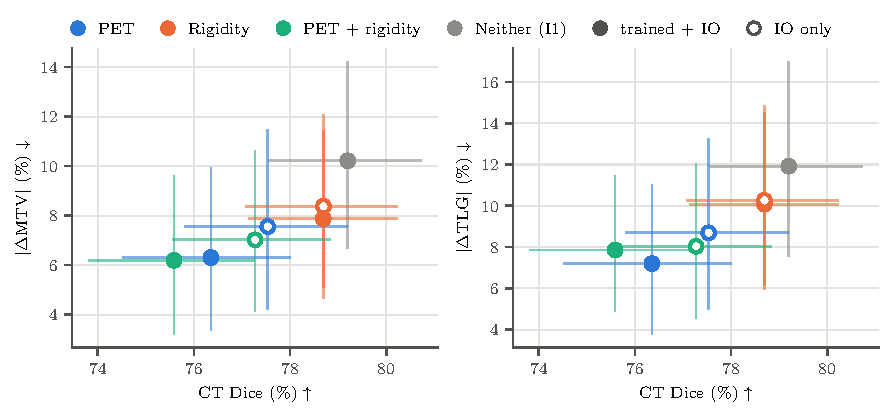
\includegraphics[width=\textwidth]{figures/q2.pdf}
\caption{Losses in training and IO versus only in IO (test set; CT Dice: 28 patients, PET: 26 patients). For each loss set, filled: network trained with the losses, then IO with them; hollow: network trained without them (T1), same IO. Grey: neither loss (I1). Points: patient means with 95\,\% patient-bootstrap confidence intervals for each method; confidence intervals for paired differences are reported in the text.}
\label{fig:q2}
\end{figure}


\subsection{Per-Lesion Volume Change}
\label{sect:res_lesions}
\todo{Text from findings.md, ``Per-lesion volume change: draft results text''.}
\begin{figure}[t]
\centering
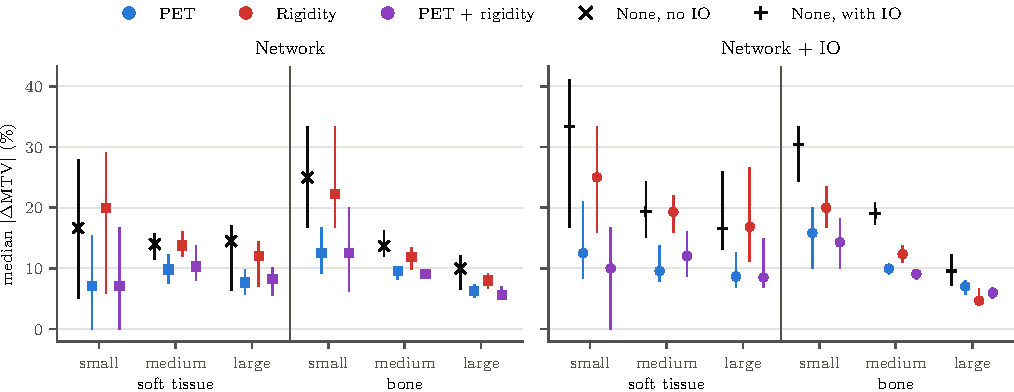
\includegraphics[width=\textwidth]{figures/lesions.pdf}
\caption{Per-lesion absolute volume change on the test set (1327 lesions from 26 patients and 30 pairs after excluding 108 components smaller than five voxels), stratified by location (soft tissue or bone-associated, with $\geq$50\,\% of the lesion on bone) and size (small $<0.5$~ml, medium $0.5$ to $<5$~ml, large $\geq5$~ml).
 Points show the median $|\Delta\mathrm{MTV}|$ per lesion; left: network output, right: instance optimization (IO) with the same losses.
 Within each size stratum, the loss groups are ordered PET, rigidity, and PET plus rigidity; squares and circles denote without and with IO, while $\times$ and $+$ denote the corresponding configurations without losses.
 Error bars: 95\,\% confidence intervals from a patient-cluster bootstrap.}
\label{fig:lesions}
\end{figure}


\subsection{Contribution of Each PET Term}
\label{sect:res_loo}
\todo{Leave-one-out table (tables/loo.tex) once L1--L4 have run.}

\subsection{Comparison with Baselines}
\label{sect:res_baselines}
\todo{Text from Table~\ref{tab:baselines}, Fig.~\ref{fig:baselines_distribution}, Fig.~\ref{fig:qualitative}: every variant of ours significantly more accurate than NiftyReg, ConvexAdam, and the affine; no folding; ranks; affine + IO reaches 52.7\,\% Dice, so the network is essential; runtimes.}
\begin{table}[t]
\centering
\caption{Comparison with baselines on the test set (28 patients, 38 follow-up$\rightarrow$baseline pairs; PET: 26 patients, 30 pairs).
 Values are mean$\pm$SD over patients (a patient's eligible pairs are averaged first).
 HD95: 95th-percentile Hausdorff distance; MTV: metabolic tumor volume; TLG: total lesion glycolysis; NDV: non-diffeomorphic volume.
 Rank: descriptive challenge significance ranking, with the 95\,\% interval of the rank over 1000 patient bootstrap samples in brackets, over all methods except Initial, which is a reference (its MTV/TLG change is 0 by construction because nothing is resampled).
 Training / IO: PET and rigidity losses (PET + rig.) used in training and in instance optimization (IO); IO ``--'': no IO, ``basic'': IO with the similarity and regularization terms only.
 $^{\dagger}$/$^{\ddagger}$: Ours + IO with PET + rig. only in IO (our method, chosen on the validation set) is significantly better/worse than this method (two-sided Wilcoxon signed-rank test on patient values, Holm-corrected over nine comparisons for CT/HD95/NDV and eight for PET within each column, $p<0.05$; NDV tested after the 0.005\,\% equivalence threshold).
 NDV is summarized as mean$\pm$SD over patients; $>$ thr. is the percentage of individual pairs with \%NDV above 0.005\,\%.
 Runtime per pair on one NVIDIA RTX A6000 (measured in the runs with the earlier scorer, same IO settings), including the affine step.
 Affine + IO: our instance optimization directly after the affine pre-registration, without the network.
 Bold: best mean among ranked methods.}
\label{tab:baselines}
\scriptsize
\setlength{\tabcolsep}{2.5pt}
\resizebox{\textwidth}{!}{%
\begin{tabular}{lllcccccccc}
\toprule
Method & Training & IO & Rank $\downarrow$ & Dice (\%) $\uparrow$ & HD95 (mm) $\downarrow$ & $|\Delta\mathrm{MTV}|$ (\%) $\downarrow$ & $|\Delta\mathrm{TLG}|$ (\%) $\downarrow$ & NDV (ppm) $\downarrow$ & $>$ thr. (\%) & Runtime (s) \\
\midrule
Initial & -- & -- & -- & 9.5$\pm$8.1$^{\dagger}$ & 44.37$\pm$21.32$^{\dagger}$ & 0.0$\pm$0.0 & 0.0$\pm$0.0 & 0$\pm$0 & 0 & -- \\
Affine & -- & -- & 8 [4--9] & 46.4$\pm$11.0$^{\dagger}$ & 14.00$\pm$4.83$^{\dagger}$ & \textbf{4.5}$\pm$4.6 & \textbf{4.4}$\pm$4.6$^{\ddagger}$ & \textbf{0}$\pm$0 & 0 & 10.4$\pm$0.3 \\
NiftyReg & -- & -- & 6 [1--8] & 70.1$\pm$5.0$^{\dagger}$ & 8.85$\pm$3.73$^{\dagger}$ & 8.7$\pm$12.8 & 10.2$\pm$16.9 & 328$\pm$885 & 21 & 107.7$\pm$24.9 \\
ConvexAdam & -- & -- & 7 [7--9] & 61.7$\pm$4.5$^{\dagger}$ & 9.16$\pm$3.14$^{\dagger}$ & 9.3$\pm$12.0 & 10.8$\pm$16.5 & \textbf{0}$\pm$0 & 0 & 11.3$\pm$0.6 \\
Affine + IO & -- & PET + rig. & 8 [4--9] & 56.6$\pm$12.1$^{\dagger}$ & 12.88$\pm$4.81$^{\dagger}$ & 5.3$\pm$4.1 & 6.8$\pm$4.0 & 0.45$\pm$0.31 & 0 & 155.5$\pm$2.6 \\
\midrule
Ours & -- & -- & 4 [3--6] & 75.5$\pm$4.7$^{\dagger}$ & 7.20$\pm$2.30$^{\dagger}$ & 10.3$\pm$9.5 & 12.5$\pm$11.1 & 0.056$\pm$0.057 & 0 & 11.0$\pm$0.4 \\
Ours & PET + rig. & -- & 5 [1--6] & 73.6$\pm$4.6$^{\dagger}$ & 7.44$\pm$2.37$^{\dagger}$ & 8.0$\pm$9.0 & 9.8$\pm$10.9 & 0.64$\pm$0.62 & 0 & 11.3$\pm$0.3 \\
Ours + IO & -- & basic & 1 [1--4] & \textbf{80.2}$\pm$4.2$^{\ddagger}$ & \textbf{6.64}$\pm$2.28$^{\ddagger}$ & 11.3$\pm$11.9 & 14.5$\pm$14.1 & 0.65$\pm$0.13 & 0 & 153.9$\pm$2.6 \\
Ours + IO & PET + rig. & PET + rig. & 3 [1--5] & 77.3$\pm$4.9$^{\dagger}$ & 7.07$\pm$2.38$^{\dagger}$ & 7.9$\pm$9.7 & 10.3$\pm$10.4 & 10.4$\pm$49.3 & 3 & 156.6$\pm$2.7 \\
Ours + IO & -- & PET + rig. & 2 [1--4] & 78.3$\pm$4.4 & 6.89$\pm$2.31 & 8.7$\pm$10.7 & 11.3$\pm$11.2 & 4.15$\pm$9.45 & 5 & 157.2$\pm$2.6 \\
\bottomrule
\end{tabular}}
\end{table}

\begin{figure}[t]
\centering
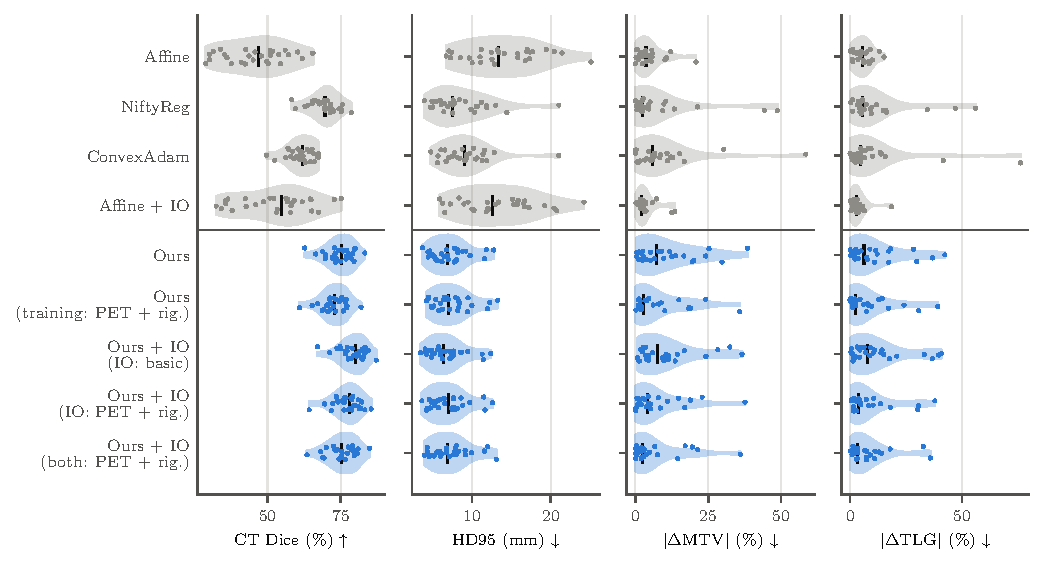
\includegraphics[width=\textwidth]{figures/baselines_distribution.pdf}
\caption{Patient-level results on the test set (CT Dice and HD95: 28 patients; PET: 26 patients; a patient's eligible pairs are averaged).
 Violins: kernel density over patients, line: median; each dot is one patient. In brackets: where the PET and rigidity losses (PET + rig.) act; basic: IO with the similarity and regularization terms only; both: training and IO.
 Initial alignment is omitted (CT Dice 9.5\,\%, HD95 44.4\,mm; MTV/TLG change 0 by construction, Table~\ref{tab:baselines}).}
\label{fig:baselines_distribution}
\end{figure}

\begin{figure}[p]
\centering
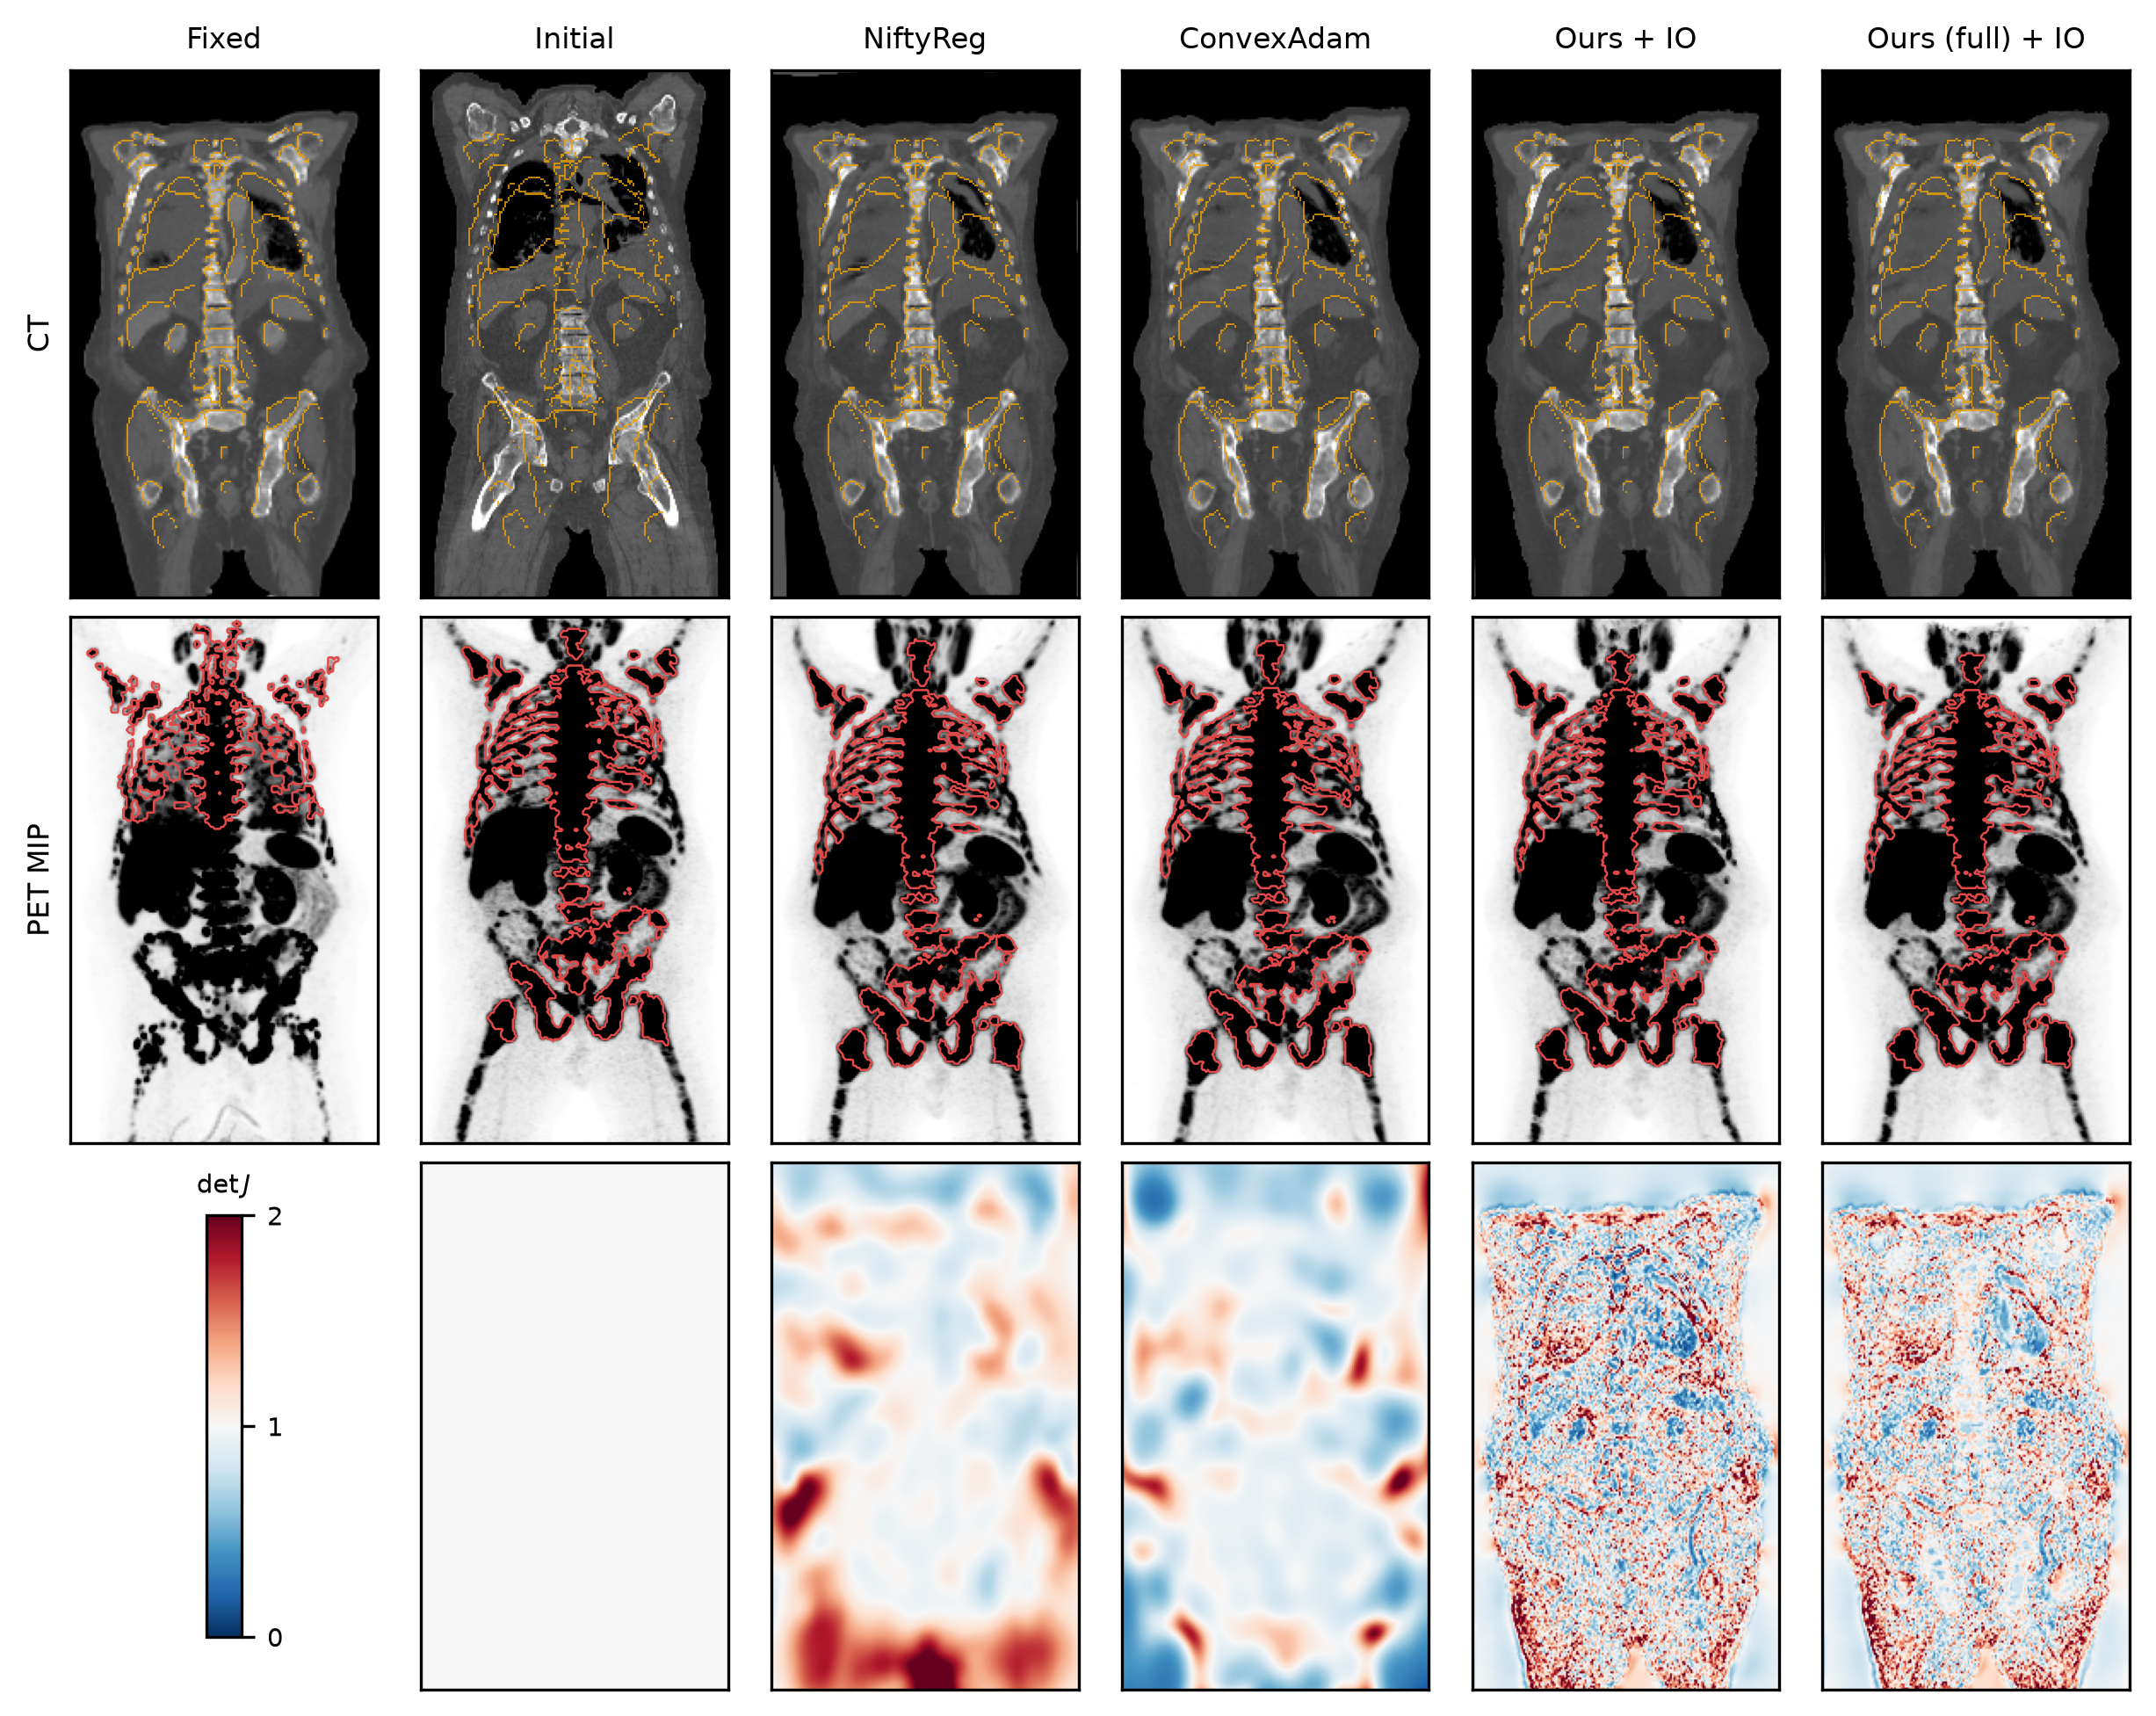
\includegraphics[width=\textwidth]{figures/qualitative.png}
\caption{Anatomical alignment example from the test set, registered by our method (PET-preservation and rigidity losses only in instance optimization [IO]); one coronal slice.
 Patient 0146 was selected for its large between-image change in lesion volume (2400 voxels at baseline and 24\,191 at follow-up).
 The example illustrates anatomical alignment and deformation.
 (a)~Fixed and (b)~moving CT images overlaid with the corresponding PET images (SUV 0--8, 35\,\% opacity) and provided lesion contours (red).
 (c,~d)~Fixed CT image (green) overlaid with the moving CT image (magenta) before~(c) and after~(d) registration; gray where they agree.
 (e,~f)~Organ labels that differ before~(e) and after~(f) registration: green where the fixed image has a label that the moving image lacks there, magenta where only the moving image is labeled; bright, medium, and dark shades for bones, organs, and muscles.
 (g)~Jacobian determinant of the fixed-to-moving transformation: white is volume-preserving (1), blue is below 1 and red is above 1; changes in the displayed warped anatomy have the opposite direction.
 (h)~Warped moving CT image overlaid with the corresponding PET image and warped lesion contours.}
\label{fig:qualitative}
\end{figure}


\subsection{Rigidity Penalties}
\label{sect:res_rigidity}
\todo{After the validation sweeps and test runs: curve of Dice vs.\ distance distortion (validation), test table with bone/soft-tissue alignment, distance distortion, NDV in bone and boundary band, stencil leakage, erosion retention. Leakage on all 560 scans: 21.2\,\% of stencil reads leave the bone; erosion keeps 35.5\,\% of bone voxels and removes 23\,\% of bones (ribs: 2.4\,\% kept, 58\,\% removed).}

\subsection{Accuracy--Preservation Trade-off}
\label{sect:res_tradeoff}
\todo{Trade-off curve (PET weight $\times\{0,0.01,0.03,0.1,0.3,1\}$) once the runs are done; mark the tuned operating point.}

\section{Discussion}
\label{sect:discussion}

Compared with network output, IO with the PET-preservation and bone-rigidity losses improved alignment by about three Dice points without a detected difference in scan-level MTV or TLG change.
Without those losses, the mean MTV and TLG changes rose after IO.
This result supports loss-guided IO when predicted lesion masks and time for per-pair refinement are available.
Applying the losses only during IO gave higher alignment accuracy than using them in both training and IO, although the paired intervals do not establish equivalent PET preservation.
The remaining scan-level change arose largely from lesions missed by the predicted masks, while individual lesions still changed substantially even with provided masks.
Bone-rigidity penalties addressed a separate anatomical aim: preserving within-bone geometry.

\subsection{Choosing Where to Apply the Losses}
Network-only registration takes about 11~s per pair on our GPU and requires only the image pair at inference.
Loss-guided IO additionally requires predicted organ and lesion masks and about 2.5~minutes per pair.
Relative to the same network output, it gained 2.9 Dice points, while the paired changes were $-1.7$ points for $|\Delta\mathrm{MTV}|$ and $-1.2$ points for $|\Delta\mathrm{TLG}|$.
No difference was detected for either PET measure.
Loss-guided IO therefore offers additional alignment when the masks and per-pair runtime are available, whereas network output provides the faster option.

Among the IO variants, applying the losses only during refinement gained 1.0 Dice points compared with using them during training and IO.
The paired intervals still allow worse MTV or TLG preservation with IO-only placement, so the result supports an accuracy gain but leaves the preservation trade-off uncertain.
Without IO, training with the losses lowered the mean registration-induced changes in lesion volume and uptake; only the MTV reduction was detected after correction.
The training losses are therefore not superseded by IO, but they serve a different setting, e.g.\ fast registration of many follow-up examinations.

One possible explanation for the IO-only result is how each stage locates lesions.
During network training, lesion labels define the preservation losses, but the trained registration network receives only images at inference and must respond to lesion-related image cues without a mask.
IO instead uses an explicit mask from a separately trained lesion-segmentation model, which can direct preservation to the predicted lesions in each pair.
This could explain why the test did not detect a preservation benefit from adding the losses during training once IO was applied.
The comparison does not test what lesion information the registration network learns, and the segmentation model cannot by itself explain the Dice advantage of IO-only placement: both IO variants use the same predicted masks.

\subsection{Limits of Lesion Preservation}
Three mechanisms must be distinguished.
First, incomplete lesion-mask coverage limits how far IO can reduce scan-level MTV and TLG change.
Second, scan-level aggregation allows growth and shrinkage of different lesions to cancel.
Third, the soft quantities optimized by the losses differ from the nearest-neighbor quantities used for evaluation.
On the predicted lesion masks that IO optimizes, the PET losses reduced volume change from 9.3\,\% to 0.8\,\%; on the provided masks, 9.3\,\% MTV and 11.8\,\% TLG change remained.
Increasing the PET weights tenfold had little effect on those measured changes.
Missed lesions were the largest measured contributor to the residual (5.2 of 9.3 MTV points and 6.2 of 11.8 TLG points), although they make up only 6\,\% of lesion volume; covered lesions still contributed 3.3 and 5.4 points.
Their weight comes from patients with little tumor volume: the metric is relative per scan and averaged over patients, and in the third of patients with the smallest lesion volume, missed lesions made up 33\,\% of the volume (23\,\% and 3\,\% in the other thirds) and caused 72\,\% of the missed-lesion contribution.
The post-hoc recall-biased mask increased lesion detection but sharply reduced precision and did not improve measured preservation (Sec.~\ref{sect:res_detection}).
The additional false-positive regions may dilute the preservation constraints over voxels outside the lesions being evaluated, so this experiment does not show that recall gains are ineffective when precision can be retained.
The diagnostic run with provided lesion masks reduced the measured changes from 9.3\,\% to 0.1\,\% for MTV and from 11.8\,\% to 4.5\,\% for TLG, while improving Dice from 78.6\,\% to 79.1\,\%.
This supports mask quality as a major limit of scan-level preservation, but uptake change remains even with provided masks, and the result does not establish that segmentation explains all residual error.

Because IO meets its objective on the predicted masks already at small weights, the PET weight mainly trades accuracy.
In the post-hoc test-set sweep, a factor of $10^{-4}$ of the training-derived weights gave the same measured MTV change while mean Dice remained 80.2\,\%, whereas the validation-selected factor ($\times0.1$) cost 1.6 Dice points and gave 1.1 points lower TLG change.
The original validation grid contained no nonzero factor below $\times0.1$, so the sweep reveals an unresolved part of the trade-off rather than a better selected setting.
An expanded low-weight sweep on validation data, followed by independent confirmation, would be required before recommending a factor below $\times0.1$.
Even with the provided masks, a ten times larger weight hardly reduced the measured MTV or TLG change.

Mask coverage does not explain the second limit: aggregate MTV and TLG changes hide how individual lesions are deformed.
Small lesions changed most in every condition, partly because a change of one or two voxels is already a large relative change.
Without the losses, IO increased the distortion of lesions, most of all of small bone-associated lesions, which tended to grow.
The rigidity loss acted mainly on bone-associated lesions, as intended, and the PET losses on both bone-associated and soft-tissue lesions; with both groups of losses, bone-associated lesions changed about as little as with the PET losses alone.
IO with the losses improved alignment without a detected difference in scan-level change from the network output, but did not reduce the change of individual lesions, not even with the provided lesion masks.
The PET losses constrain the total volume and uptake of a scan, which can remain nearly unchanged while single lesions grow or shrink.
Indeed, provided masks reduced scan-level MTV change to 0.1\,\%, while the median per-lesion change remained 13.5\,\%.

Adding per-lesion terms to the connected components of the predicted mask reduced per-lesion change on the validation set but provided no consistent benefit on the test set.
In the intended test-time setting, these terms constrain only the eight largest predicted components with at least 20 voxels, leaving smaller and additional components unconstrained.
They also act on predicted components, which can miss lesions or merge and split them, and use the same soft, linearly warped masks as the scan-level terms, whose change differs from the evaluated one (Sec.~\ref{sect:res_loo}).
A separate diagnostic using the provided lesion masks also failed to reduce the median per-lesion change, although these masks are unavailable in the intended setting.
A per-lesion constraint may therefore require constraints for small lesions and a closer surrogate of the nearest-neighbor evaluation.

The leave-one-out experiment exposes the third mechanism: the optimized surrogate does not always track the evaluated endpoint.
In IO, the Jacobian terms carried the preservation, whereas removing the volume term $\mathcal{L}_{\mathrm{MTV}}$ or the uptake term $\mathcal{L}_{\mathrm{TLG}}$ improved $|\Delta\mathrm{TLG}|$ by 1.1 and 2.0 points, respectively, and removing $\mathcal{L}_{\mathrm{MTV}}$ also gained 0.6 Dice points.
Both terms act on the soft, linearly warped mask, whose change differs from the nearest-neighbor change that is evaluated.
This is one possible explanation for the result, but the experiment does not show that interpolation mismatch caused it.
We retained all four terms because this leave-one-out analysis used the test set and the configuration had been fixed beforehand.
A closer surrogate or a reduced set of terms would require selection on validation data and confirmation on independent data.

\subsection{Interpreting the Evaluation}
The significance-based ranking of the challenge was decided mainly by accuracy: differences in alignment between methods are consistent across patients and reach significance, whereas differences in MTV and TLG vary strongly between patients and rarely do.
On the validation set, the ranking would consequently have chosen our variant without any of the losses; we therefore selected our method with a rule that weighs preservation within a fixed Dice tolerance (Sec.~\ref{sect:tuning}).
Preservation metrics should therefore be read together with anatomical alignment; neither higher CT Dice nor lower MTV/TLG change alone establishes which registration is more useful for a clinical task.
The MTV and TLG endpoints compare the same follow-up acquisition before and after warping, so they isolate change introduced by registration rather than biological change between examinations.
This study does not define or validate a threshold at which such change alters lesion tracking, response classification, or another clinical decision.
The reported differences should therefore be interpreted as technical fidelity measures rather than demonstrated clinical benefit.
The scan-level MTV and TLG changes are also an incomplete measure of preservation: they sum over all lesions of a scan, so a lesion that grows can cancel one that shrinks.
With provided lesion masks, IO reduced the scan-level volume change to 0.1\,\%, although single lesions still changed by a median of 13.5\,\%; a near-zero scan-level change therefore does not show that each lesion was preserved.
Per-lesion changes, which do not cancel between lesions, should complement the scan-level metrics, in particular for tasks that follow individual lesions, such as lesion-level response assessment.

Both the measured alignment and preservation of IO depend in part on the labels it uses.
On the predicted organ labels, IO raised Dice from 79.0\,\% to 88.0\,\%, but on the provided labels it raised Dice only from 75.5\,\% to 78.6\,\%.
For lesions, the PET losses reduced MTV change measured on the predicted masks nearly to zero, while lesions missed by those masks received no direct constraint.
Within this segmentation-based evaluation, the diagnostic lesion-mask run shows that better lesion masks can improve the reported PET metrics; organ-mask quality may also affect the measured alignment.
Outside this setting, label overlap and the change of MTV and TLG are proxies: what matters clinically is whether registration supports downstream tasks such as lesion tracking, response assessment, or dose accumulation.
Future work should therefore evaluate registration on such tasks and clinical endpoints rather than optimize further for segmentation-based metrics.

The baseline comparison also illustrates the role of deformation regularity.
At the pair level, NiftyReg exceeded the folding threshold on 5 of 38 validation pairs and 8 of 38 test pairs (21\,\%), with up to 0.37\,\% NDV.
The ranking selected its least-regularized setting because accuracy separated the settings more than folding; a setting chosen on the validation set did not transfer to new patients.
The selected method exceeded the 0.005\,\% NDV threshold on two test pairs and the training-plus-IO variant on one, with a maximum of 0.026\,\% NDV across our reported variants.

\subsection{Bone Rigidity}
Finite-difference rigidity penalties face a trade-off at bone boundaries: their stencils read across the boundary (21\,\% of the reads), so they also stiffen the surrounding tissue, and eroding the bones to avoid this leaves most of the skeleton unconstrained at this resolution (35.5\,\% of bone voxels kept, ribs 2.4\,\%).
The per-bone rigid fit avoids both, because it compares each bone's displacement with its best rigid motion and needs no derivatives.
It produced the lowest within-bone distance distortion among the tested penalties, although it does not optimize that measure, and increased soft-tissue Dice by 0.9 points relative to IO without rigidity.
The cost of rigid bones is lower bone Dice, possibly because a rigid bone cannot follow differences between the automatic bone labels of the two examinations as closely as a freely deforming one.
Whether this lower overlap reflects worse alignment or an inability of a rigid bone to follow inconsistencies between the automatic bone labels cannot be decided from label overlap alone.
The lower within-bone distance distortion shows better preservation of bone shape, but it does not determine whether the bone is placed correctly.

Although about two thirds of the lesion voxels lie on bone labels (63\,\% in the training and 67\,\% in the test scans), adding a rigidity penalty on top of the PET losses did not measurably improve lesion volume or uptake preservation in this comparison.
Rigidity alone did improve particular PET endpoints in Fig.~\ref{fig:q2}: it reduced network-output $|\Delta\mathrm{MTV}|$ and IO $|\Delta\mathrm{TLG}|$ relative to the corresponding unconstrained variants.
Three factors may contribute to the absence of a detected additional benefit on top of the PET losses.
First, the PET losses already constrain the predicted lesions.
Second, the bones were not made rigid at the scale of the lesions: the remaining rigid-fit residual of 1.4 to 2.3~mm is about half a voxel, enough to move the boundary voxels of lesions that span only a few voxels, whereas an exactly affine transformation changed bone-associated lesions by a median of only 1.0\,\%.
Third, the scan-level metrics are dominated by missed lesions, by cancellation between lesions, and by a few patients with large changes (Sec.~\ref{sect:res_detection}).
The per-bone rigid fit therefore reduces measured within-bone distance distortion, with a measured cost in bone Dice.
The present measures do not establish whether it improves bone placement, and a further PET-preservation benefit may require bones that are rigid to within a fraction of a voxel.

\subsection{Limitations}
The study uses a single cohort with 28 test patients, so small differences, in particular in MTV and TLG, could not be resolved, and generalization to other scanners and tracers is untested.
The images were resampled to about $2.7\times2.7\times3.3$~mm, at which many lesions consist of few voxels and small lesions are dominated by discretization.
The organ labels used for evaluation are themselves automatic (TotalSegmentator), and the lesion labels used by IO are predictions with a Dice of about 0.5, which, as shown above, limits preservation in IO.
All patients, including the test patients, were part of the challenge data with which the earlier version of the method was developed; the test patients were not used for any decision in the present study.
We studied one network architecture, and we measured the change caused by registration, not its effect on clinical decisions such as response assessment.

\section{Conclusion}
\label{sect:conclusion}

With predicted lesion masks, instance optimization with PET-preservation and bone-rigidity losses improved anatomical alignment without a detected difference in scan-level MTV or TLG change relative to network output.
Without those losses, the mean MTV and TLG changes rose after instance optimization.
Applied only during instance optimization, the losses gave higher alignment accuracy than when they were also used in training; the present test set did not resolve whether preservation differs between these placements.
Without instance optimization, training with the losses lowered the mean MTV and TLG changes at a cost in alignment; only the MTV reduction was detected after correction.
Missed lesions accounted for much of the residual scan-level change in the mask-coverage analysis.
Even with provided masks, substantial changes to individual lesions remained despite a near-zero scan-level MTV change.
Better lesion masks may reduce scan-level error, while per-lesion evaluation is needed to reveal changes that whole-scan metrics hide.
For bones, a per-bone rigid fit produced the lowest within-bone distance distortion among the tested penalties, at a cost in bone Dice.
Adding rigidity on top of the PET losses did not produce a detected further reduction in lesion-measurement change, although rigidity alone improved particular PET endpoints relative to the unconstrained variants.


\subsection*{Disclosures}
The authors declare that there are no financial interests, commercial affiliations, or other potential conflicts of interest that could have influenced the objectivity of this research or the writing of this paper.

\subsection*{Code, Data, and Materials Availability}
All experiments use the publicly available training data of the Learn2Reg 2026 PSMAReg challenge~\cite{ref_learn2reg_alessa,ref_learn2reg_hansen}, which is adapted from the PSMA-PET-CT-Lesions dataset in The Cancer Imaging Archive~\cite{ref_psmaregdata} (DOI: 10.7937/r7ep-3x37).
The private test data of the challenge were not used.
The patient-level split into training, validation, and test sets is provided with the code.
\todo{Code repository link (training, IO, evaluation, split, and trained weights).}

\subsection*{Acknowledgments}
F.K.\ and J.A.S.\ are partially supported by the German Federal Ministry of Research, Technology and Space (DECIPHER-M, 01KD2420G).
A.R.\ is supported by funding from the Free State of Bavaria (StMGP) as part of the project ``KI-gestützte multi-modale Diagnostik und stratifizierte Therapie für Endometriose (EndoKI)''.
D.M.L.\ and J.A.S.\ received funding from Helmholtz Imaging, a platform of the Helmholtz Information \& Data Science Incubator.
\todo{Funding E.C.}
L.F.\ was partially funded by the Intramural Research Funding Grant ``AI-driven Longitudinal Lesion Tracking'' of the Faculty of Medicine, University of Augsburg, by the Bavarian Center for Cancer Research as part of the Lighthouse ``Local Therapies'', and by the Bavarian Ministry of Economic Affairs, Regional Development and Energy (StMWi) under grant number DIK-2310-0004//DIK0556/02.
An AI assistant was used for language editing of the manuscript; the authors reviewed and take responsibility for all content.
The use of AI tools for code generation is described in Sec.~\ref{sect:training}.

\bibliography{references}
\bibliographystyle{spiejour}

\listoffigures
\listoftables

\end{spacing}
\end{document}
